\documentclass[../../../Main.tex]{subfiles}
\begin{document}

This subsection describes the implementation and reasoning behind the strategy for efficiently visiting all rooms using a roadmap.\\
\\
Goal:
\begin{itemize}
    \item An efficient strategy to visit all rooms of the environment given the occlusion map.
\end{itemize}
\subsubsection{Reasoning}
There is a number of different ways to achieve the goal of an efficient mapping strategy.
The goal itself is considered to have two main parts.
The first part is building a roadmap to provide the "best" way to move around in the map for the robot.
A roadmap could in principle be enough to achieve the goal if the robot only needed to move from one start to one goal.
As the robot needs to visit all rooms, there would have to be multiple goal nodes implemented.
This could technically solve the problem, but it wouldn't necessarily be very efficient unless the
shortest way around the map got hard coded into the roadmap by placing a sequence of q-goals in the order of the shortest path.
This solution, however, would be very inefficient and not very flexible, as it only fits one map and only one problem. \\
This leads to the second part of the solution: A graph search.
The roadmap essentially provides vertices and edges that combines the vertices already,
which makes a shortest path algorithm like Dijkstra's or A* ideal for solving part two of the problem. \\
The idea is to use a brushfire decomposition to create a Voroni diagram that will provide the base graph.
The brushfire/Voroni algorithm has been picked as it seemed a fairly straightforward way to create a roadmap.
The Dijkstra method was picked over A* even though the A* method is considered superior to Dijkstra, because Dijkstra seemed fairly straightforward and is simpler to implement.
\subsubsection{Implementation and discussion}
In the following subsection the implementation will be explained and discussed. \\
As will soon be apparent, we did not manage to get the Dijkstra working in time, as there was some issues with the roadmap most likely stemming from the brushfire decomposition.
This means that our method of visiting all rooms became quite less efficient which will be
explained in more detail later in the subsection.
\subsubsection*{Brushfire $\&$ Voroni}
The roadmap implementation in this project consists of two main parts:
\begin{itemize}
  \item Generating a brushfire diagram
  \item Decomposing it to obtain the Voroni diagram's vertices and edges
\end{itemize}
Both parts are implemented in a class called BrushfireAL.
The brushfire algorithm was in itself very easy to implement. To ease the process of generating the brushfire diagram, the map has been preprocessed so all black pixels has been changed from their normal pixel value\footnote{0} to 1 and all white pixels from 255 has been changed to 0.
The map has gone through the OpenCV threshold function to make sure that all pixels are either white or
black as black represents an obstacle to be avoided and white free space. \\
The brushfire algorithm in itself consists of two functions, the first one checks a white pixel's eight neighbouring pixels to see what their pixel value is. If one or more of those neighbours are black, the value of the white pixel is set to 2. If not, the other function checks the lowest value that is higher than 0 and increments it with one.
After having run through the whole map, a brushfire diagram as can be seen in figure \ref{fig:brsuhfire_1}.
\begin{figure}[H]
  \centering
  \includegraphics[width=15cm]{\main/afsnit/rob/roadmap/pictures/brushfire_1.png}
  \caption{The figure shows the generated brushfire. The edges and vertices are already present but not very visible. A path through the image can be observed as the whitest path connect all rooms}
  \label{fig:brsuhfire_1}
\end{figure}
The Voroni diagram is almost there, however the "best" path between all rooms and pathways need to be made more clear.
The way to decompose a brushfire algorithm to obtain a Voroni diagram, is by following the highest gradient between obstacles around the map and connect the patches when one or more of these highest gradient paths intersect with each other. It also comes from all corners that are not "just" an obstacle.
As will be evident in figure \ref{fig:voroni_diagram}
it has not worked completely, as not all paths are connected.
One path is missing its link to a path directly beneath it.
Some of the paths have also become thicker than is to be expected as the critical points on which the paths are build should only be one-two pixel wide.
This occurs as a pixel can not be split up into a half, so if the distance between two obstacles are an odd number, the gradient would end up being two pixels wide.\\
\begin{figure}[H]
  \centering
  \includegraphics[width=15cm]{\main/afsnit/rob/roadmap/pictures/brushfire_2.png}
  \caption{The figure shows the Voroni diagram without the vertices clearly marked. As can be observed it has not turned out perfect with a discontinuity between the top right room and the path beneath it}
  \label{fig:voroni_diagram}
\end{figure}
Adding the vertices also turned out to be difficult as the implemented version of the algorithm falsely found some corners to be considered vertices.
It does also detected multiple vertices on an edge coming from some corners, see figure \ref{fig:voroni_diagram_nodes}.
The reason for this is believed to stem from a faulty logic when deciding what is considered a vertex and what is not after having generated the brushfire diagram. The first iteration of converting  a vertex was only marked if it had at least four neighbours being the same value as itself.
\begin{figure}[H]
  \centering
  \includegraphics[width=15cm]{\main/afsnit/rob/roadmap/pictures/voroni_n.png}
  \caption{The figure shows the Voroni diagram with the vertices clearly marked. As can be observed it has not turned out perfect with a discontinuity between the top right room and the path beneath it}
  \label{fig:voroni_diagram_nodes}
\end{figure}

% ------------------------------------

The Voroni diagram can still be very useful as the extra vertices should, in principle, not hinder an efficient graph search. The disadvantage is that the graph has become larger without providing any extra useful information.\\

The next iteration is using the generated vertices and edges for a graph search.
\subsubsection*{Dijkstra}
The Dijkstra algorithm is implemented in its most basic form with one Class called Dijkstra. \\
It has been implemented using a priority queue to keep track of the shortest path between vertices.
All vertices are pushed onto the priority queue with their known distance set to infinity beside the source node that has a distance of 0.
The class has another couple of help functions, addEdge(), given two vertices and the distance between them, it creates an edge between them, and efficientWay(), which will be described below. \\

The Dijkstra itself works pretty well and, provided that all edges between all vertices has been added using the addEdge() function, it will return the shortest path between the starting node and all other vertices. This in itself does not create the solution to reach our goal, but This but outlines the two main difficulties to solve:
\begin{itemize}
  \item How to add the edges between all vertices.
  \item Utilizing the output of the Dijkstra algorithm or rewriting it to fit our purpose.
\end{itemize}
 The first problem to solve is adding all vertices and edges generated from the roadmap to the Dijkstra class.
 Unfortunately because of the issues in generating the Voroni diagram, extracting the vertices and the length of the edge connecting them proved very difficult.
 It has yet to work properly. This means there is no real test to show that the principle works beside showing that there is a roadmap and there is a Dijkstra algorithm.
 The issues are thought to be partly because of the double "pathing" explained in the subsection before and as can be observed on figure \ref{fig:voroni_diagram}.
 The another issue is getting the proper vertices sorted from the false positive ones. The ones that occurred on the edge between a corner and a proper vertex interfered with obtaining the length of some edges connecting the real vertices and not the fake ones. It was attempted to only obtain the "real" vertices, however those failed. It came close but some of the important vertices were always lost in the filtering process. A third  issue is that one path between two vertices are missing from the Voroni diagram, figure \ref{fig:voroni_diagram_nodes}.
\\

The second problem was getting an efficient way of visiting all rooms. This is what the supporting function efficientWay() meant to solve. It has not been implemented as the time ran short. The idea behind it was to alter the main function generateDijstra() to add the distance from source to all nodes and the nodes that was visited in order to go from source to the node in question to a vector. \\
The efficientWay() needs this vector in order to find an efficient way through the map. Every node gets a weight variable, that gets incremented by 1 every time it has been used to visit another vertex from source. There will be two vertices with a very high count as they are in each side of the hallway connecting the robots starting point and hence the source vertex with the two sides of the map, see figure \ref{fig:map_node1}. The vertices should also be divided into two "types", 1 and 2. This refers to which vertex next to the source they pass coming from source.
\begin{figure}[H]
  \centering
  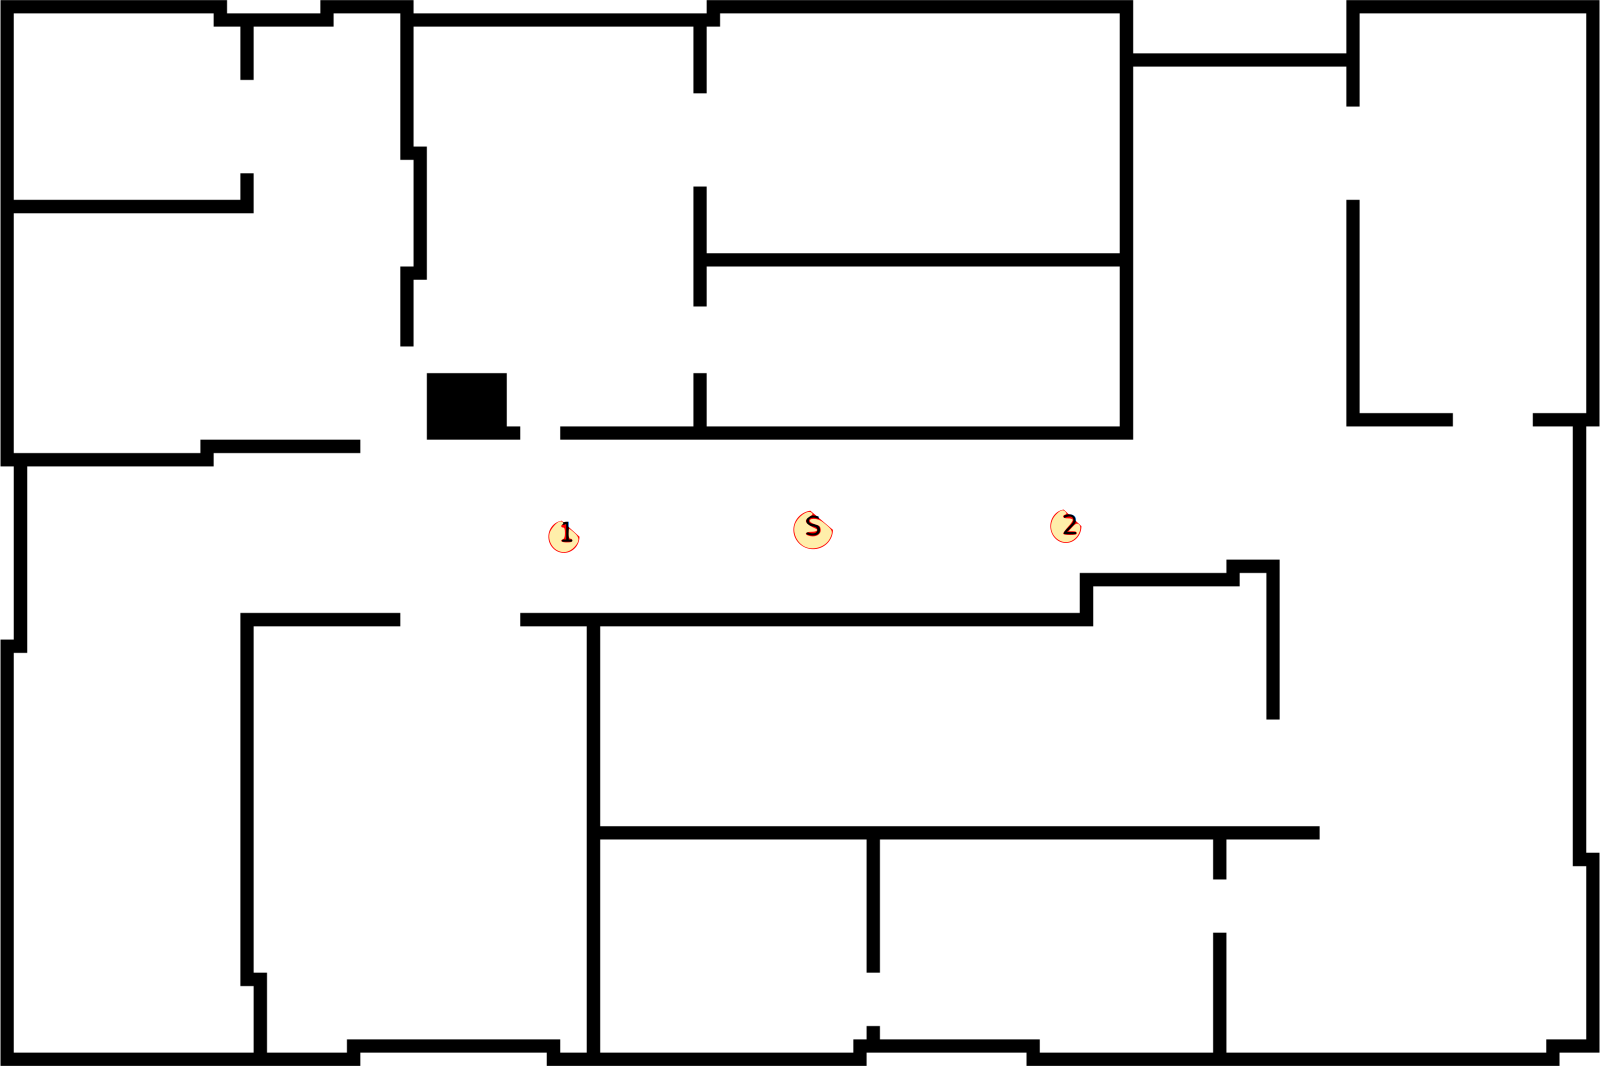
\includegraphics[width=15cm]{\main/afsnit/rob/roadmap/pictures/floor_plan.png}
  \caption{The figure shows the map with the source vertex, marked with S, and the two most visited nodes, marked with an 1 and 2}
  \label{fig:map_node1}
\end{figure}
The robot will arbitrarily start with either the left or right most weighted node (1 or 2), as starting with either side does not change its efficiency.
The robot should not pass the source node again before it has visited all vertices in its current side of the map.\\
It chooses the next vertex to visit by inspecting whether or not the adjacent nodes has been visited.
If more than one is unvisited, it'll choose the one with the lowest weight.
If all adjacent vertices has been visited, it'll pick the vertex with the highest count, as the chance of it being in contact with another unvisited vertex is highest.\\

\subsubsection{Conclusion $\&$ Improvement}
The goal was not reached as some of the issues with the Voroni diagram was not resolved, which means that the Dijkstra and roadmap could not be combine to form the wanted strategy.\\
The issues can of course be resolved, however it is suspected that a complete rewrite of the brushfire class is needed.
If it was possible to start over, instead of using half of the method of brushfire decomposition to obtain the Voroni diagram, it might be as simple just using the algorithm that Voroni is based on and measure the distance between all obstacles and create the path that way.
It would make troubleshooting easier as for now the issue could lie both on the brushfire generation and in the way to Voroni diagram is created. \\
It is expected that the function efficientWay(), if implemented, could solve the problem regarding an efficient strategy to visit all rooms. Dijkstra does need a roadmap as else it does not have a clear path to follow between each obstacle.
\end{document}
